\section{Design Overview and Choices}
The general idea of the Mobility Feature Package is to provide an API that is easy to use for the application programmer, such that the features can be computed with as few lines of code as possible. This requires closing off the API to a large degree which has the upside of leaving very little possibility of error in the hands of the programmer. However, it is indeed a balancing act, in which swaying too much to one side can have consequences. 

\subsection{Design Process}
The design of the package API went through two main iterations which consisted of many smaller iterations. Mainly, the difference between the final iteration and the previous one is the amount of logic for managing historical data contained within the package. Previously most of this work was done by the application programmer 'outside the package' i.e. when writing a specific application. A major step in making the decision of moving logic inside the application was done after developing the study app discussed in chapter \ref{chapter:06}. For this application the previous iteration was used, and it became glaringly apparent that too much work had to be done by the programmer. The final iteration is the one discussed in this thesis including the choices and lessons learned on the way of designing and developing it.

\subsection{Managing Complexity}
Designing an API is a balancing act of managing complexity. This means decisions have to be made in regards to what logic is kept internal and what should be kept external (i.e. left to the application programmer). As mentioned, location data is required to be collected to compute features which is done through a location service API. It is a possibility to move this data collection inside the package, but it has been chosen not to do so, to ensure the long term maintainability and modularity of the package. The location service depends on the platform and programming framework of choice and leaving this particular choice to the programmer therefore makes sense. To take the middle road, it was chosen to include a data storage API in the package, which allows the programmer to easily store the collected data. As such, the only steps of the process left to the application programmer is to collect location data, store it on the device (through the Mobility Features Package API) and compute features when they are needed. Getting around using a custom location plugin can be done by converting between \textit{Data Transfer Objects} (DTOs) \footnote{\url{https://martinfowler.com/eaaCatalog/dataTransferObject.html}} which in this case are simply objects holding location data, i.e. latitude, longitude and a timestamp. The DTOs considered are that of the programmers location plugin and that of the Mobility Features Package, namely \textit{LocationSample}.

\subsection{Component Overview}
Some components of the package should be external, i.e. accessed and used by the application programmer and some should be kept internal. For this external/internal paradigm, class access is used in most object oriented programming languages. Class access refers to the access that the programmer has to a given class, i.e. whether it is private or public, or whether it can be instantiated. This can be applied to to ensure that the the programmer uses the package in the manner in which it was intended. If all classes were publicly available and could be instantiated, many edge cases arise in which the programmer may produce errors. In a worst case scenario this may lead to an app  crashing in production where valuable data is lost as a result. This can even happen in spite of proper documentation and keeping certain components private is therefore very desirable. Figure \ref{fig:component-diagram} depicts the architecture of the Mobility Features Package, the type face indicates the access: 
 
 \begin{figure}[h]
    \centering
    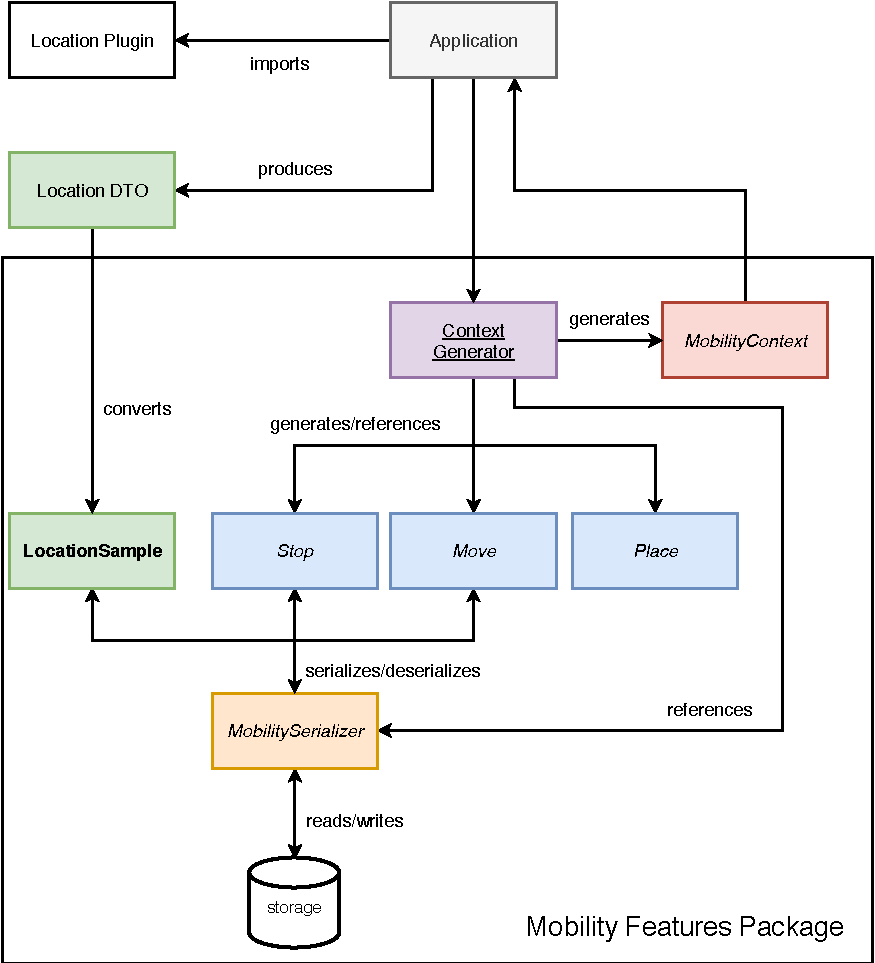
\includegraphics[width=\textwidth]{images/diagrams/api-diagram.pdf}
    \caption{Component diagram for the Mobility Feature Package displaying the access of each component when implemented as a class}
    \label{fig:component-diagram}
\end{figure}
 
A bold typeface indicates the class can be instantiated by the user and is publicly available. An underlined typeface indicates the class is static and therefore cannot be instantiated but is publicly available to the programmer. A class with an italic typeface is a class which cannot be directly instantiated by the user but is available through the API. \\
 
\textbf{Bold:} Contents of this DTO are transferred to the equivalent DTO of the \textit{Mobility Features Package}, namely \textit{LocationSample} which is workaround for allowing the programmer to use any location service API. The programmer therefore has public access to the \textit{LocationSample} class and can instantiate it.\\

\textbf{Underlined:} The sole static class in the diagram is the \textit{ContextGenerator} class which is the main interface for the application programmer. This class contains a reference to the \textit{MobilitySerializer} class that allows the user to serialize \textit{Location Samples}, which the user can use to get an instance of the \textit{MobilitySerializer}. This \textit{ContextGenerator} component is also responsible for instantiating  Mobility Context objects, which is done by loading Location Samples stored via the \textit{MobilitySerializer} (as well as Stops and Moves if applicable) in order to compute the \textit{MobilityContext}. Concretely, a \textit{ContextGenerator} generates a \textit{MobilityContext} which contains a series of features including \textit{Stops}, \textit{Places} and \textit{Moves}.\\

\textbf{Italic:} Common for the \textit{MobilityContext} as well as \textit{Stops}, \textit{Places} and \textit{Moves} is that neither can directly be directly instantiated by the programmer, but they can be generated through the \textit{ContextGenerator} component. \\



